\documentclass{beamer}
\usepackage[utf8x]{inputenc}
\usepackage[T2A]{fontenc}
\usepackage[english,russian]{babel}

\usetheme{mybeamer}

\usepackage[most]{tcolorbox}

\title{Влияние точности входных параметров моделей ядерных реакций на предсказанные выходы $r$-процесса}
\subtitle{Магистерская диссертация}
\author{Негребецкий В.В.}
\institute{МГУ им. М.В. Ломоносова, физический факультет,\\
кафедра общей ядерной физики\\
\vspace{1em}
\textnormal{Научный руководитель: к.ф.-м.н. Стопани К.А.}
}
\date{}

\begin{document}
  \frame[noframenumbering] {
    \titlepage
  }

  \frame{
    \frametitle{Образование тяжелых элементов}
    \small
    Особенности $r$-процесса:
    \begin{itemize}
      \item Экстремальные условия ($T \approx 1-5$~ГК)
      \item Участие \textbf{сильно нейтроноизбыточных} ядер
    \end{itemize}
    \center
    \includegraphics[width=0.9\textwidth]{../pics/tracks.pdf}
    
    \vspace{0.3cm}
    Изучение сводится к \textbf{компьютерному моделированию}.
  }

  \frame{
    \frametitle{Моделирование нуклеосинтеза}
    \small
    Система уравнений нуклеосинтеза: 
    \begin{equation*}
    \displaystyle 
    \frac{d y_i}{d t} = \sum_{k \in K_i} \pm {\color{blue}\lambda_k} \prod_{l \in L_k} y_l
    \end{equation*}
    
    Особенности задачи:
    \begin{itemize}
      \item Огромная размерность ($\sim 7800$ изотопов и $\sim 10^5$ реакций)
      \item Сверхжесткость системы уравнений 
      \item Неопределенность астрофизических параметров
      \item Недостаток данных о задействованных экзотических ядрах, \\
        \textbf{их характеристики приходится получать из моделей}
    \end{itemize}
    

    \begin{tcolorbox}[colback=blue!10, colframe=blue!10]
      Ядерные данные влияют на моделирование $r$-процесса через 
      величины астрофизических 
      \textbf{скоростей реакций $\color{blue}\lambda_k$}.
    \end{tcolorbox}
  }

  \frame{
    \frametitle{Астрофизические скорости реакций}
    \small
    \textbf{Скорость реакции $\color{blue}\lambda_k$} --- это вероятность протекания реакции на единицу времени на единицу концентрации каждой исходной частицы.
    
    \begin{equation*}
      \displaystyle
      \lambda(T) = \int_0^\infty \sigma(E) \rho(E, T) dE,
    \end{equation*}
    где $\rho(E, T)$ --- энергетическое распределение.
    
    \vspace{0.5cm}

    \begin{itemize}
      \item Для $r$-процесса $\sigma(E)$ можно получить лишь из теоретических моделей (статистический подход Хаузера--Фешбаха).
      \item Для этого нужно характеристики нейтроноизбыточных ядер (например, массы), которые \textbf{тоже получают из моделей}.
    \end{itemize}
    
    
    \begin{tcolorbox}[colback=blue!10, colframe=blue!10]
      Неопределенности ядерных моделей непосредственно\\
      влияют на расчеты нуклеосинтеза через скорости реакций.
    \end{tcolorbox}
  }

  \frame{
    \frametitle{Модели масс экзотических ядер}
    \small
    Нами рассмотрены разные подходы к описанию ядер:
    \begin{itemize}
      \item HFB-24 \textit{\scriptsize Goriely et al 2013} --- микроскопическая модель
      \item FRDM2012 \textit{\scriptsize M\"oller et al 2016} --- макро-микроскопическая
      \item LMR2021 \textit{\scriptsize Владимирова и др 2022} --- метод локальных соотношений
    \end{itemize}
      
      \includegraphics[width=\textwidth]{../pics/deviations-scaled.pdf}
  }

  \frame{
    \frametitle{Расчет сечений и скоростей $(n,\gamma)$}
    \small
    Вычисления выполнены с помощью пакета TALYS \textit{\scriptsize Koning et al 2019}. 
    \vspace{0.2cm}

    \center
    \begin{minipage}{0.42\textwidth}
      \center
      $^{236}\text{Pb}$
      \includegraphics[width=\textwidth]{../pics/cs_pb236.pdf}
      \includegraphics[width=\textwidth]{../pics/ng_fit_pb236.pdf}
    \end{minipage}
    \begin{minipage}{0.42\textwidth}
      \center
      $^{237}\text{Pb}$
      \includegraphics[width=\textwidth]{../pics/cs_pb237.pdf}
      \includegraphics[width=\textwidth]{../pics/ng_fit_pb237.pdf}
    \end{minipage}
    
    Скорости $(n,\gamma)$ $\color{blue}\xrightarrow{\text{пакет ratelib}}$
    база данных REACLIB \textit{\scriptsize Cyburt et al 2010}
  }

  \frame{
    \frametitle{Скорости $\beta$-распадов}
    \small
    \begin{itemize}
    \item Для каждой реакции $(n,\gamma)$ нужно внести в базу данных $\beta$-распад продукта, чтобы не было накопления нестабильных ядер. 
    \item Если в REACLIB нет такого распада, получаем его аппроксимацией.
    \end{itemize}

    \center
    \begin{minipage}{0.49\textwidth}
      \center
      Тербий, $Z = 65$
      \includegraphics[width=\textwidth]{../pics/decay_fit65.pdf}
    \end{minipage}
    \begin{minipage}{0.49\textwidth}
      \center
      Свинец, $Z = 82$
      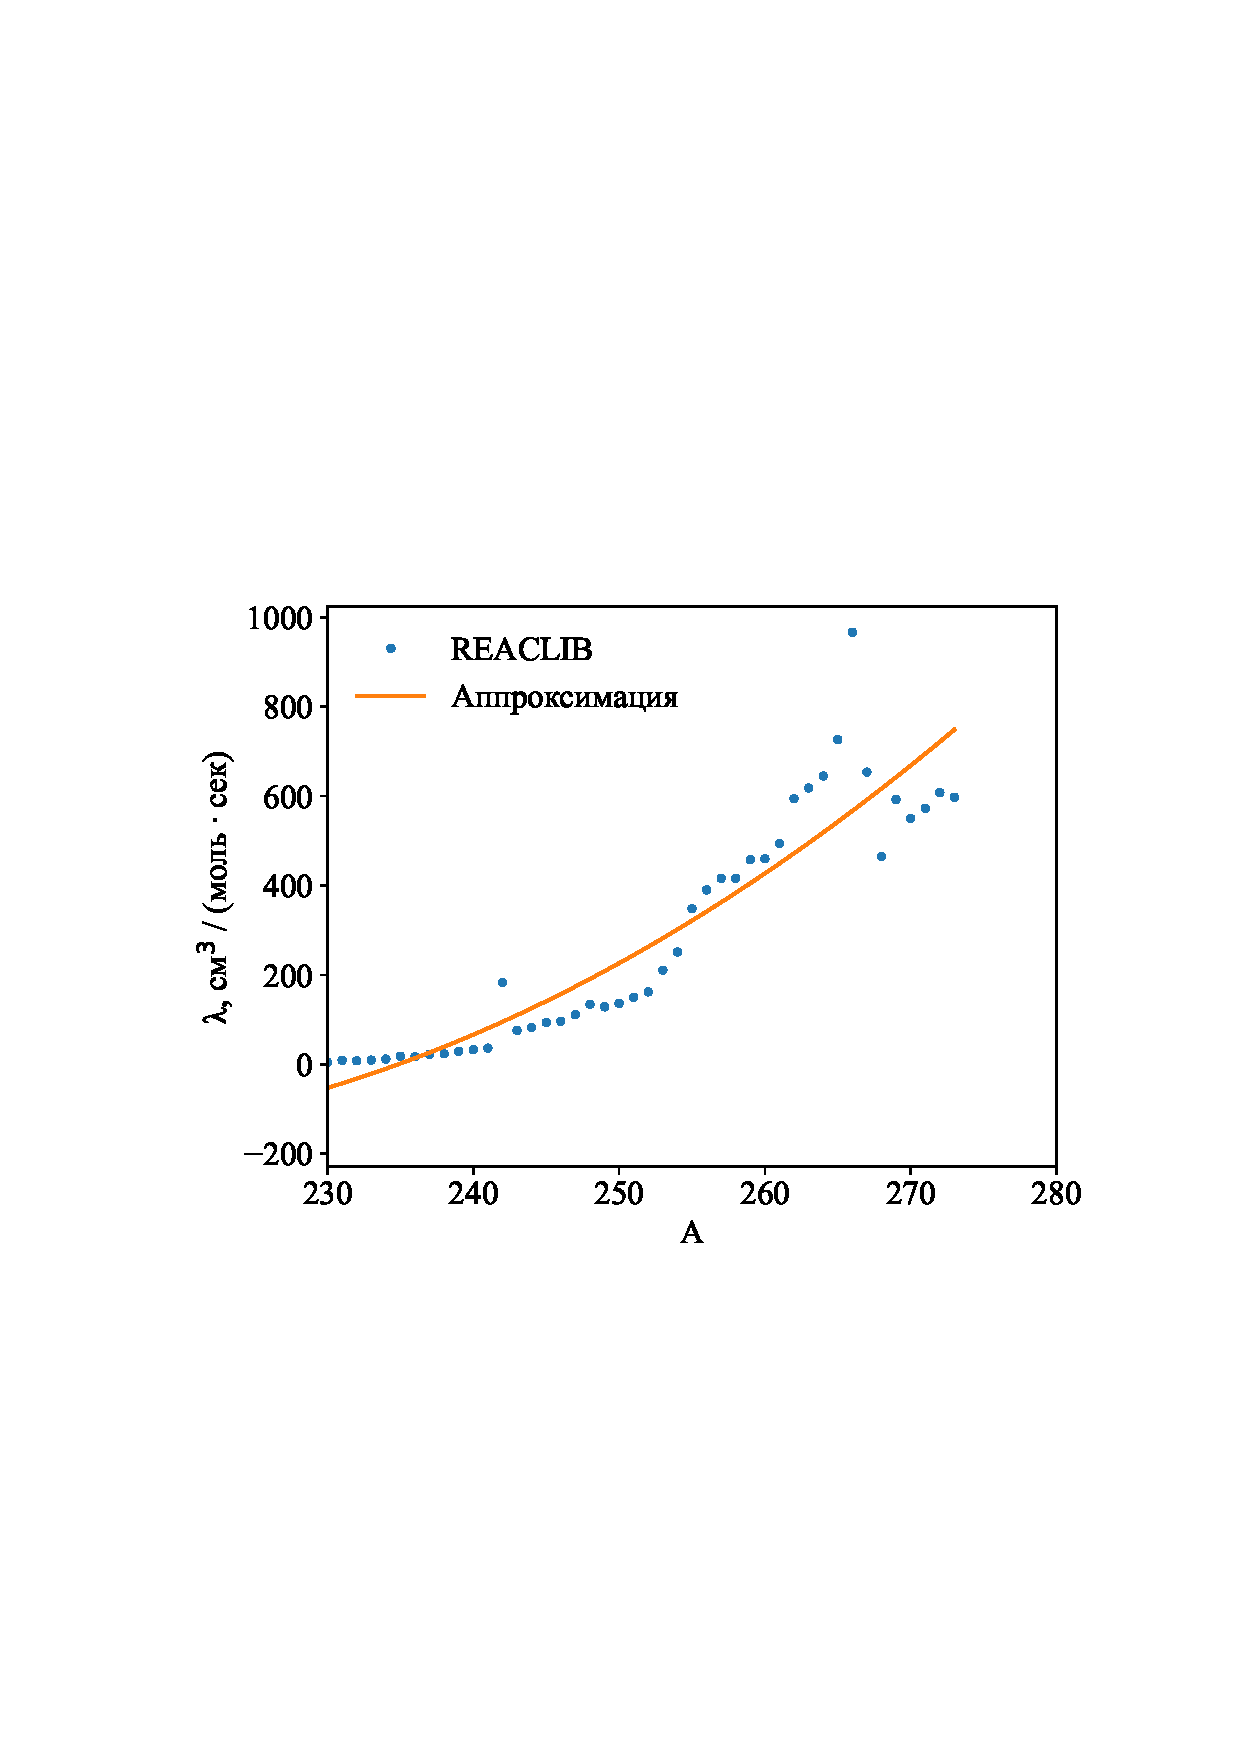
\includegraphics[width=\textwidth]{../pics/decay_fit82.pdf}
    \end{minipage}
    
    Модельная функция --- правило Сарджента: $\lambda_\beta \sim Q_\beta^5$
  }
  
  \frame{
    \frametitle{Моделирование $r$-процесса}
    \small
    Модель $r$-процесса в выбросах при слиянии нейтронных звезд.
    \begin{itemize}
    \item Начальные условия: 
      $T = 6$~ГК, $Y_e = 0.1$, $s = 10~\frac{k_B}{\text{барион}}$.
    \item Вещество выброса расширяется с постоянной скоростью.
    \item Исходный состав вещества определяется условием равновесия.
    \end{itemize}
    
    \center
    \includegraphics[width=0.8\textwidth]{../pics/distr_1000.pdf}
    
    Расчет с помощью библиотеки SkyNet \textit{\scriptsize Lippuner Roberts 2017}.
  }
  
  \frame{
    \frametitle{Эволюция выходов $r$-изотопов}
    \small \center
    \begin{minipage}{0.49\textwidth}
      \center
      ${}^{179}\text{Tb}$
      \includegraphics[width=\textwidth]{../pics/y_65_179.pdf}
      ${}^{190}\text{Tb}$
      \includegraphics[width=\textwidth]{../pics/y_65_190.pdf}
    \end{minipage}
    \begin{minipage}{0.49\textwidth}
      \center
      ${}^{180}\text{Tb}$
      \includegraphics[width=\textwidth]{../pics/y_65_180.pdf}
      ${}^{191}\text{Tb}$
      \includegraphics[width=\textwidth]{../pics/y_65_191.pdf}
    \end{minipage}
  }

  \frame{
    \frametitle{Результаты}
    \begin{itemize}
      \item С помощью TALYS и ядерных моделей HFB-24, FRDM2012 и LMR2021 получены скорости реакций $(n,\gamma)$ $r$-процесса.
      \item Из этих данных с помощью нашего пакета ratelib составлены базы данных астрофизических реакций.
      \item Эти базы данных использованы для моделирования $r$-процесса в слиянии нейтронных звезд на основе библиотеки SkyNet.
      \item Изучено влияние выбора массовой модели на симуляцию $r$-процесса.
    \end{itemize}
  }
  
  \usebeamertemplate{endpage}

  \frame{
    \frametitle{Распространенность ядер в Солнечной системе}
    \small
    \begin{itemize}
      \item Легкие ядра образуются в реакциях звездного горения.
      \item Синтез ядер за железом энергетически невыгоден.
      \item Тяжелых изотопов действительно много меньше, чем легких.
    \end{itemize}

    \center
    \includegraphics[width=\textwidth]{../pics/lodders_vs_ame.pdf}

    \begin{tcolorbox}[colback=blue!10, colframe=blue!10]
      \center
      Образование тяжелых ядер обеспечено $s$- и $r$-процессами.
    \end{tcolorbox}
  }

  \frame{
    \frametitle{Подробнее о модели LMR2021}
    \small
    \center
    Связь энергий связи четырех соседних ядер через $np$-корреляции:
    $\Delta_{np}(N,Z) = B(N,Z) + B(N-1,Z-1) - B(N,Z-1) - B(N-1,Z)$
    
    \vspace{0.5cm}
    Аппроксимация:
    $\Delta^\text{аппр}_{np} = \alpha A^{\beta}$

    \includegraphics[width=0.9\textwidth]{../pics/delta_np-scaled.pdf}

  }

  \frame{
    \frametitle{Нейтронный захват за границей существования}
    \small
    Таблицы теоретических ядерных масс обычно выходят за границы существования.
    Учитывать ли реакции $(n,\gamma)$ для ядер с $B_n < 0$?

    \center
    \includegraphics[width=0.75\textwidth]{../pics/rates_vs_A_tb-scaled.pdf}
  }
  
  \frame{
    \frametitle{Подробнее об аппроксимации слабых распадов}
    \small
    В области нейтронного избытка обычный $\beta$-распад подавлен распадами с вылетом нейтронов. В $r$-процессе любой недостаток нейтронов в ядре очень быстро компенсируется.
   
    \center
    \includegraphics[width=\textwidth]{../pics/decays_tb.pdf}
    
    \scriptsize
    Скорости слабых распадов \textbf{тербия} из базы данных REACLIB.
  }
  
  \frame{
    \frametitle{Влияние массовой модели на температуру}
      \small
      $r$-процесс может нагревать среду за счет $\beta$-распадов. Как выбор массовой модели влияет на этот нагрев?

    \center
    \includegraphics[width=\textwidth]{../pics/temp.pdf}

    Наши три базы данных отличаются по распадам только вблизи границы отделения, поэтому разница малозаметна, но она есть.
      
  }
\end{document}
